% mlr3fairness currently has two preprocessing methods, one postprocessing method and several fairness adjusted models implemented. We decide to use a reweighing methods that works with assigning weights to the observations to equalise the distribution of $P(Y|PA)$.
% The inprocessing method is a fairness-adjusted logistic regression implemented in mlr3fairness inspired by Zafar et. al. This method optimises for statistical parity (independence). The postprocessing method we choose aims for equalised odds and it works by randomly flipping a subset of predictions with pre-computed probabilities in order to satisfy equalised odds constraints.
\subsubsection*{Bias and the feedback loop}
\begin{figure}
    \centering
    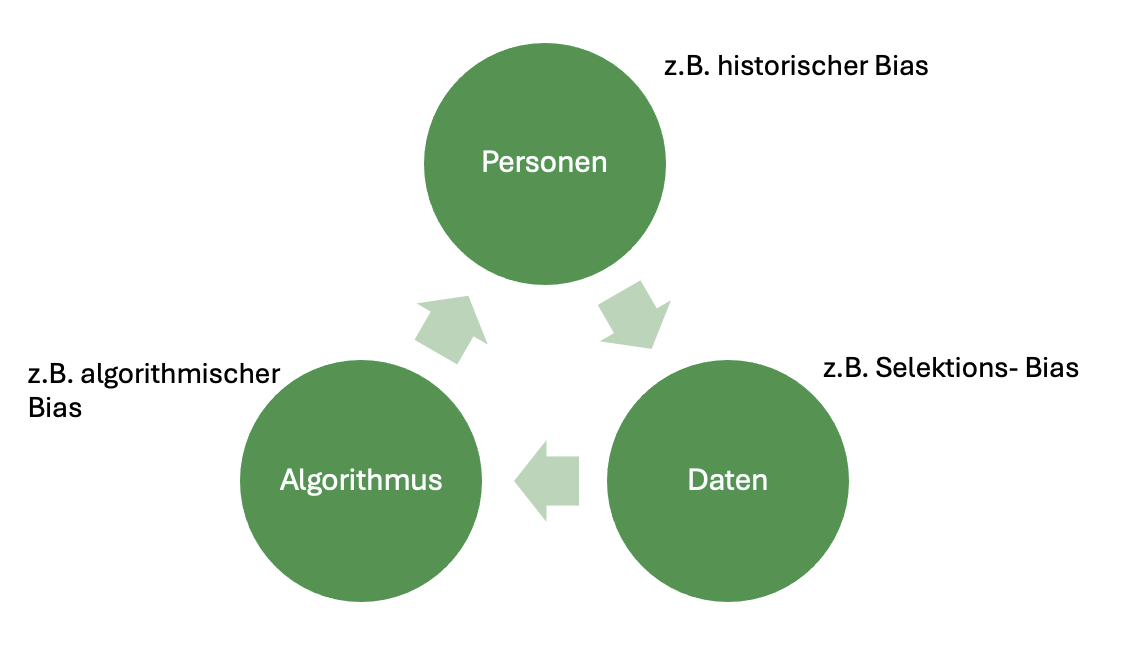
\includegraphics[width=0.7\textwidth]{../figures/bias_loop.png}
    \caption{The bias loop.}
    \label{fig:bias_loop}
\end{figure}

Usually fairness is a concern in the first place, because the algorithm should be implemented as an ADM to assist decision-making in some way. As such it could influence if someone gets admitted to college, gets a loan or is released from prison. The algorithm does not exist in isolation, but is embedded in a loop with data and the user.
We make the circumstances of a decision measurable by collecting data. The algorithm learns from this data to make an optimal prediction, on which the decision-makers base their judgement on \autoref{fig:bias_loop}. At each step of this loop, bias can be introduced in the process and, more dangerous, be amplified as the algorithm influences decision-making on a large scale.
This means that every fairness project comes with the task to understand where the data comes from and how exactly the algorithm will be deployed in practice. With this in mind we can maybe explain they complex and ambigous picture drawn by SQF studies.

\subsubsection*{Conclusion}
In conclusion, the questions of fairness for SQF is difficult.
Before any fairness intervention, we have to formulate a clear fairness question. It is something entirely different to ask if the stop, question, and frisk practice (as a whole) is fair or whether a classifier to predict the arrest of a person trained on SQF data is fair? Or whether a classifier trained to predict the possession of a weapon trained on SQF data is fair?
The exact question we formulate leads us to look at different aspects of the data. In this paper we got a first idea of the answer to the first questions by comparing certain characteristics of the SQF population to the population of NYC as a whole (descriptive analysis) and find that the two populations do differ. But does it make sense to want the SQF sample be representative for whole NYC or does it not make more sense to want it to be representative of the population of criminals in NYC?
Here we see a closer match in racial distributions. This, however, is by far not enough to claim the fairness of the police practice. Crime statistics have to be read with caution. They are influenced by many factors, including the amount of police in a certain area, the socio-economic status of the population and the trust in the police. Historical discrimination leads to lower socio-economic, lower socio-economic status comes with higher crime rates, higher crime rates lead to more police in the area, more police in the area lead to more reported crime. Crime statistics are embedded in a broad context and do not necesarily reflect objective inherent truths but our social and economic system.
We can cite \cite{goel2016} who approach the question in a more wholeistic way, account for complex factors and come to the conclusion that SQF is over-targetting PoC.
As we saw in our own case study and \cite{Badr2022DTFANSP} also find, is that this does not mean a classifier trained on SQF data violates group fairness. Depending on the task some classifiers might perform better on the historically disadvantaged group while others in fact discriminate against them.
With this study we do not claim to give the answer to fairness in SQF but the goal was to show the readers the complexity of the situation/ give critical perspective/ show different approaches to fairness in SQF. As many datasets, this one comes with a great backstory (socio-economic context, historical biases) and problems (group imbalance, ...) and all of this is entangled. We should be aware of this otherwise it might misinterpretation of results.


